\chapter{Costi}

\section{Calcolo dei costi}

La parte teorica di questo progetto si basa sulla stima di costi di esecuzione delle operazioni sulle differenti opzioni di organizzazione dei documenti, per calcolare cio' 
abbiamo bisogno di alcune formule che andro qui ad elencare:  

\subsection{NL}
    \begin{equation*}
        \begin{aligned}
        NL &=\floor*{\frac{NK * len(k) + NR * len(p)}{D * u}}
        \end{aligned}
        \end{equation*}
\subsection{g}
    \begin{equation*}
        \begin{aligned}
        g &=\ceil*{\frac{D - len(p)}{2 * (len(k) + len(p))}}
        \end{aligned}
        \end{equation*}
\subsection{h}
Il calcolo per l'altezza del b-tree relativo agli indici degli attributi verrebbe normalmente calcolato attraverso questa formula, nel nostro caso di studio l'altezza e' stata approssimata a 3.
    \begin{equation*}
        \begin{aligned}
        \floor*{\log_{(2*g + 1)}{NL}} \leq h \leq \ceil*{\log_{(g + 1)}{\frac{NL}{2}}}
        \end{aligned}
        \end{equation*}
\subsection{NP}
    \begin{equation*}
        \begin{aligned}
        NP &=\floor*{\frac{NR * len(t)}{D * u}}
        \end{aligned}
        \end{equation*}
\subsection{Costo del nested loop}
In cui ho R relazione esterna e S relazione interna
\begin{itemize}
    \item senza predicato di selezione 
    \begin{equation*}
        \begin{aligned}
        NP_R + NR_R * NP_S
        \end{aligned}
        \end{equation*}
    \item con predicato di selezione 
    \begin{equation*}
        \begin{aligned}
            NP_R + (sel(pred) * NR_R) * costo(S)
        \end{aligned}
        \end{equation*}
\end{itemize}
\subsection{Indice clustered}
    \begin{equation*}
        \begin{aligned}
            Costo(S)&= (h -1) + \floor*{\frac{1}{NK} * NL} +  \floor*{sel(pred) * NP}
        \end{aligned}
        \end{equation*}
\subsection{Indice unclustered}
    \begin{equation*}
        \begin{aligned}
            Costo(S)&= (h -1) + \floor*{\frac{1}{NK} * NL} + 1 + \phi(\frac{NR}{NK}, NP)
        \end{aligned}
        \end{equation*}

\begin{center}
    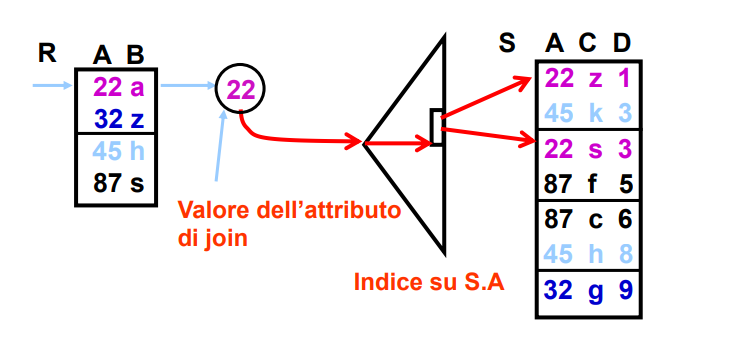
\includegraphics{nestedLoop.png}
\end{center}


\begin{center}
    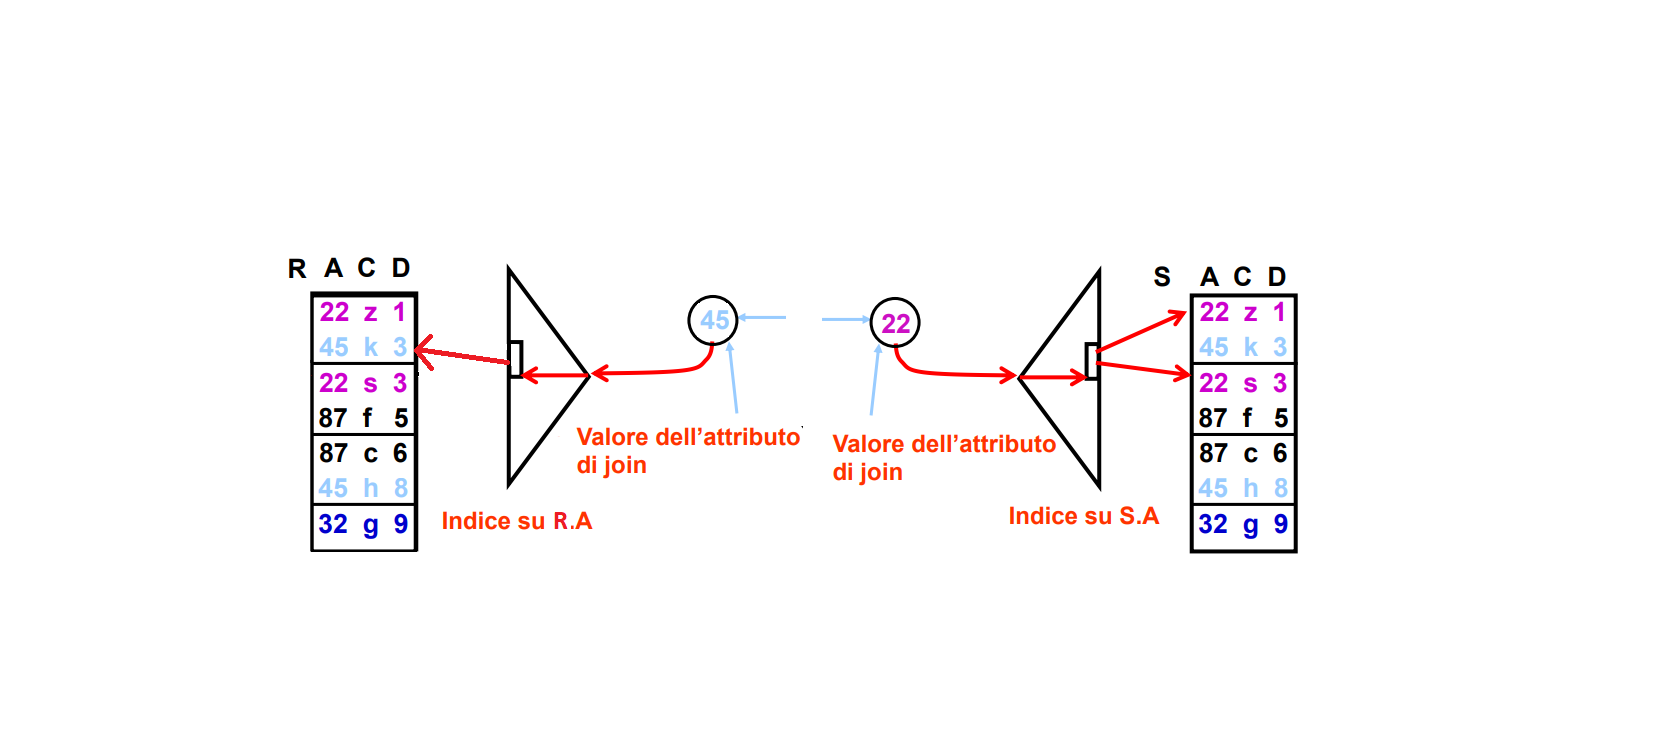
\includegraphics[scale=0.4]{nestedLoop 2 indici.png}
\end{center}